% ============================================================================
% Homework 1 -- Solutions.  Same preamble as hw01.tex plus tikz/listings and a
% blue `solution' environment.  Self-contained; compiles with pdflatex.
% ============================================================================
\documentclass[10pt]{article}

\usepackage[a4paper, margin=2.2cm]{geometry}
\usepackage{amsmath, amssymb}
\usepackage[dvipsnames]{xcolor}
\usepackage{array}
\usepackage{enumitem}
\usepackage{tikz}
\usepackage{listings}
\usepackage{needspace}
\usepackage[hidelinks]{hyperref}

\definecolor{ruleink}{RGB}{18, 68, 140}
\definecolor{solink}{RGB}{20, 60, 170}

\setlength{\parindent}{0pt}
\pagestyle{plain}

\AtBeginDocument{%
  \abovedisplayskip=5pt plus 1pt
  \belowdisplayskip=5pt plus 1pt
  \abovedisplayshortskip=3pt
  \belowdisplayshortskip=3pt}

\lstset{basicstyle=\ttfamily\small, columns=fullflexible, keepspaces=true,
  xleftmargin=1em, aboveskip=4pt, belowskip=4pt}

% ---- one problem -----------------------------------------------------------
\newcommand{\problem}[2]{%   points, title
  \par\bigskip
  {\color{ruleink}\rule{\textwidth}{1pt}}\par\nobreak\vspace{3pt}
  {\large\bfseries #2}\hfill{\normalsize\bfseries(#1 points)}\par\nobreak\vspace{4pt}}

\newlist{parts}{enumerate}{1}
\setlist[parts]{label=(\alph*), leftmargin=2.2em, itemsep=3pt}

% ---- solution block ----------------------------------------------------------
\newenvironment{solution}
  {\par\smallskip\begingroup\color{solink}\textbf{Solution.}\ }
  {\endgroup\par}

\begin{document}

\begin{center}
  {\large OL7014 Integer Programming}\\[3pt]
  {\Large\bfseries Homework 1 --- Solutions}\\[4pt]
  {\small \textbf{Due Sep 15, start of class}}
\end{center}
\medskip\hrule\medskip

Problem 6 is an optional bonus (20 points).

% ================================================================ Problem 1
\problem{20}{Problem 1. Reading and writing the language}

A transport aircraft is being loaded for a resupply flight. Three cargo types:

\begin{center}
\begin{tabular}{l|ccc}
              & water pallet & fuel drum & medical pallet \\ \hline
 value (pts)  & 5 & 4 & 7 \\
 weight (t)   & 2 & 3 & 1 \\
 volume (m$^3$) & 3 & 1 & 2 \\
\end{tabular}
\end{center}

The aircraft carries at most $60$ t and $55$ m$^3$. Orders require that \emph{exactly}
$4$ medical pallets fly. For this problem cargo is divisible --- fractional pallets may
be manifested. The goal is to maximize total value.

\begin{parts}
\item \textbf{(6 pts)} Define the decision variables and write the problem as a scalar
  LP: objective plus constraints, one line each, with a few words saying what each
  constraint enforces.

\begin{solution}
Let $x_1, x_2, x_3 \ge 0$ be the numbers of water pallets, fuel drums, and medical
pallets loaded.
\[
\begin{aligned}
  \max\quad & 5x_1 + 4x_2 + 7x_3 && \text{total value} \\
  \text{s.t.}\quad & 2x_1 + 3x_2 + x_3 \le 60 && \text{weight limit (t)} \\
                   & 3x_1 + x_2 + 2x_3 \le 55 && \text{volume limit (m$^3$)} \\
                   & x_3 = 4 && \text{exactly four medical pallets} \\
                   & x_1, x_2, x_3 \ge 0 && \text{no negative cargo}
\end{aligned}
\]
\end{solution}

\item \textbf{(8 pts)} Put your LP in the standard form
  $\max\, c^{\top}x$ s.t.\ $Ax \le b$ from Week 1. Write out $c$, $A$, $b$ with
  numbers in them. Remember the dictionary: an equality becomes \emph{two} inequality
  rows, and nonnegativity gets its own rows. Report the dimensions of $A$.

\begin{solution}
$x_3 = 4$ becomes $x_3 \le 4$ and $-x_3 \le -4$; each $x_j \ge 0$ becomes $-x_j \le 0$.
\[
c = \begin{pmatrix} 5 \\ 4 \\ 7 \end{pmatrix}, \qquad
A = \begin{pmatrix}
  2 & 3 & 1 \\
  3 & 1 & 2 \\
  0 & 0 & 1 \\
  0 & 0 & -1 \\
  -1 & 0 & 0 \\
  0 & -1 & 0 \\
  0 & 0 & -1
\end{pmatrix}, \qquad
b = \begin{pmatrix} 60 \\ 55 \\ 4 \\ -4 \\ 0 \\ 0 \\ 0 \end{pmatrix}
\qquad
\begin{array}{l}
  \scriptstyle\text{weight} \\ \scriptstyle\text{volume} \\
  \scriptstyle x_3 \le 4 \\ \scriptstyle x_3 \ge 4 \\
  \scriptstyle x_1 \ge 0 \\ \scriptstyle x_2 \ge 0 \\ \scriptstyle x_3 \ge 0
\end{array}
\]
$A$ is $7 \times 3$.
\end{solution}

\item \textbf{(3 pts)} Is the feasible set a polyhedron? Is the problem convex?
  One sentence each.

\begin{solution}
Yes: $\{x : Ax \le b\}$ is an intersection of finitely many half-spaces, which is
a polyhedron by definition. Yes: a polyhedron is convex and the objective is linear,
so the problem is convex.
\end{solution}

\item \textbf{(3 pts)} Orders change: only \emph{whole} pallets and drums may fly
  ($x \in \mathbb{Z}^3$). Which of your answers in (c) change, and to what?

\begin{solution}
Both become \emph{no}. The feasible set $\{x \in \mathbb{Z}^3 : Ax \le b\}$ is a
finite set of lattice points: $(0,0,4)$ and $(1,0,4)$ are feasible but their midpoint
$(\tfrac12,0,4)$ is not, so it is not convex, hence not a polyhedron, and the problem
is not convex.
\end{solution}
\end{parts}

% ================================================================ Problem 2
\problem{20}{Problem 2. Convexity, by pictures}

No formal proofs in this problem. All you need is the \emph{segment test} from
lecture --- a set is convex when the straight segment between any two of its points
stays inside --- plus a pencil and a ruler. Label your drawings.

\begin{parts}
\item \textbf{(7 pts)} Draw two convex sets in $\mathbb{R}^2$ whose \emph{union} is
  not convex: mark two points of the union and the point on their segment that
  escapes it. Then \emph{try} to draw two convex sets whose \emph{intersection} is
  not convex. After a few honest attempts, state in one sentence what you believe
  to be true about intersections --- no proof needed, just your pictures.

\begin{solution}
\par\medskip
\begin{center}
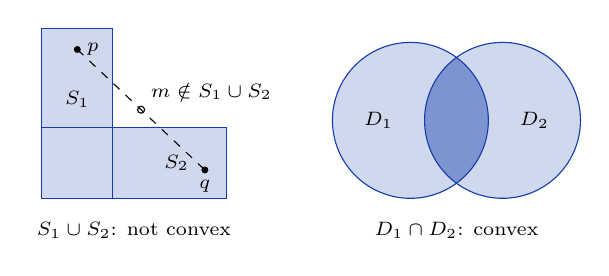
\begin{tikzpicture}[scale=0.9, every node/.style={font=\scriptsize}]
  % union: L-shape
  \fill[solink!20] (0,0) rectangle (1,2.4);
  \fill[solink!20] (0,0) rectangle (2.6,1);
  \draw[solink] (0,0) rectangle (1,2.4);
  \draw[solink] (0,0) rectangle (2.6,1);
  \node at (0.5,1.4) {$S_1$};
  \node at (1.9,0.5) {$S_2$};
  \fill (0.5,2.1) circle (1.4pt) node[right] {$p$};
  \fill (2.3,0.4) circle (1.4pt) node[below] {$q$};
  \draw[dashed] (0.5,2.1) -- (2.3,0.4);
  \draw (1.4,1.25) circle (1.4pt) node[above right] {$m \notin S_1 \cup S_2$};
  \node at (1.3,-0.45) {$S_1 \cup S_2$: not convex};
  % intersection: lens
  \begin{scope}[xshift=5.2cm, yshift=1.1cm]
    \fill[solink!20] (0,0) circle (1.1);
    \fill[solink!20] (1.3,0) circle (1.1);
    \begin{scope}
      \clip (0,0) circle (1.1);
      \fill[solink!55] (1.3,0) circle (1.1);
    \end{scope}
    \draw[solink] (0,0) circle (1.1);
    \draw[solink] (1.3,0) circle (1.1);
    \node at (-0.45,0) {$D_1$};
    \node at (1.75,0) {$D_2$};
    \node at (0.65,-1.55) {$D_1 \cap D_2$: convex};
  \end{scope}
\end{tikzpicture}
\end{center}
Left: $S_1$, $S_2$ are convex, but $p \in S_1$, $q \in S_2$ and the midpoint $m$
of their segment lies in neither, so the union fails the segment test.
Right: every attempt fails --- two rectangles meet in a rectangle, two disks in a
lens, both convex. Belief: \emph{the intersection of two convex sets is always convex.}
\end{solution}

\item \textbf{(7 pts)} Draw the Week 1 toy
  $P = \{\, (x,y) \ge 0 \;:\; x + 3y \le 10, \ 3x + y \le 10 \,\}$ and mark all the
  lattice points $X = P \cap \mathbb{Z}^2$. Now run the segment test on $X$: pick
  two points of $X$ whose segment passes through a point that is not in $X$, and
  label that escaping point with its coordinates. What did the single line
  ``$\in \mathbb{Z}$'' do to convexity?

\begin{solution}
\par\medskip
\begin{center}
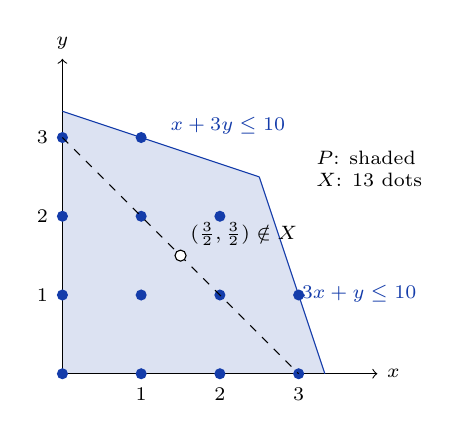
\begin{tikzpicture}[scale=1.0, every node/.style={font=\scriptsize}]
  \fill[solink!15] (0,0) -- (10/3,0) -- (2.5,2.5) -- (0,10/3) -- cycle;
  \draw[->] (0,0) -- (4,0) node[right] {$x$};
  \draw[->] (0,0) -- (0,4) node[above] {$y$};
  \foreach \i in {1,2,3} { \draw (\i,0.06) -- (\i,-0.06) node[below] {\i};
                           \draw (0.06,\i) -- (-0.06,\i) node[left] {\i}; }
  \draw[solink] (0,10/3) -- (2.5,2.5) node[midway, above right] {$x+3y \le 10$};
  \draw[solink] (10/3,0) -- (2.5,2.5) node[midway, below right] {$3x+y \le 10$};
  \foreach \p in {(0,0),(1,0),(2,0),(3,0),(0,1),(1,1),(2,1),(3,1),(0,2),(1,2),(2,2),(0,3),(1,3)}
    \fill[solink] \p circle (2pt);
  \draw[dashed] (0,3) -- (3,0);
  \draw[fill=white] (1.5,1.5) circle (2pt) node[above right] {$(\tfrac32,\tfrac32) \notin X$};
  \node[anchor=west, align=left] at (3.1,2.6) {$P$: shaded\\ $X$: 13 dots};
\end{tikzpicture}
\end{center}
$(0,3)$ and $(3,0)$ are in $X$, but the midpoint of their segment, $(\tfrac32,\tfrac32)$,
is not an integer point. The line ``$\in \mathbb{Z}$'' destroyed convexity: $P$ is
convex, $X = P \cap \mathbb{Z}^2$ is not.
\end{solution}

\item \textbf{(6 pts)} Same picture, one question: for a max problem, why can the
  LP relaxation's optimal value $z_{\mathrm{LP}}$ never be \emph{smaller} than the
  IP's $z_{\mathrm{IP}}$? Answer in one or two sentences, no notation needed.
  (Lecture's hint: deleting the ``$\in \mathbb{Z}$'' line only \emph{enlarges} the
  set of allowed plans.)

\begin{solution}
Every plan the IP allows (each dot) is also allowed by the LP (it lies in the shaded
region), so the LP chooses from a larger menu that contains the IP's best plan --- it
can match that plan, so it can never do worse.
\end{solution}
\end{parts}

% ================================================================ Problem 3
\problem{20}{Problem 3. Relax, round, regret}

A patrol packs a rucksack that carries $W = 24$ kg. Ammo boxes weigh $5$ kg and are
worth $8$ points each; med kits weigh $7$ kg and are worth $11$ points each. Any
nonnegative integer count of each may be packed:
\[
\begin{aligned}
  \max\quad & 8x + 11y \\
  \text{s.t.}\quad & 5x + 7y \le 24 \\
                   & x, y \in \mathbb{Z}_{+}
\end{aligned}
\]

\begin{parts}
\item \textbf{(5 pts)} Solve the LP relaxation graphically: draw the feasible region,
  list every vertex with its objective value, and report the LP optimum
  $(x^{\star}, y^{\star})$ and $z_{\mathrm{LP}}$.

\begin{solution}
The relaxation $5x + 7y \le 24$, $x, y \ge 0$ is a triangle.
\par\medskip
\begin{minipage}{0.5\linewidth}\centering
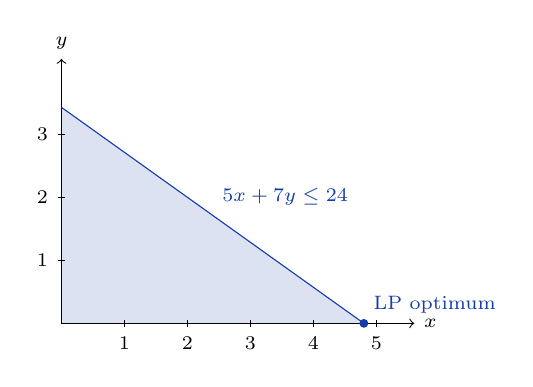
\begin{tikzpicture}[scale=0.8, every node/.style={font=\scriptsize}]
  \fill[solink!15] (0,0) -- (4.8,0) -- (0,24/7) -- cycle;
  \draw[->] (0,0) -- (5.6,0) node[right] {$x$};
  \draw[->] (0,0) -- (0,4.2) node[above] {$y$};
  \foreach \i in {1,...,5} \draw (\i,0.06) -- (\i,-0.06) node[below] {\i};
  \foreach \i in {1,2,3} \draw (0.06,\i) -- (-0.06,\i) node[left] {\i};
  \draw[solink] (4.8,0) -- (0,24/7) node[midway, above right] {$5x+7y \le 24$};
  \fill[solink] (4.8,0) circle (2pt) node[above right] {LP optimum};
\end{tikzpicture}
\end{minipage}%
\begin{minipage}{0.5\linewidth}\centering
\begin{tabular}{c|c}
 vertex & $z = 8x + 11y$ \\ \hline
 $(0,0)$ & $0$ \\
 $(\tfrac{24}{5}, 0) = (4.8, 0)$ & $38.4$ \\
 $(0, \tfrac{24}{7}) \approx (0, 3.43)$ & $\tfrac{264}{7} \approx 37.71$
\end{tabular}
\end{minipage}
\par\medskip
LP optimum: $(x^\star, y^\star) = (4.8, 0)$, $z_{\mathrm{LP}} = 38.4$.
\end{solution}

\item \textbf{(5 pts)} Round the LP optimum: list \emph{every} candidate obtained by
  taking $\lfloor\cdot\rfloor$ or $\lceil\cdot\rceil$ in each coordinate, check each
  for feasibility in a table (as in lecture), and report the best \emph{feasible}
  rounded value.

\begin{solution}
$x \in \{\lfloor 4.8 \rfloor, \lceil 4.8 \rceil\} = \{4, 5\}$; $y^\star = 0$ is already
an integer, so the $2^2$ combinations collapse to two candidates:
\begin{center}
\begin{tabular}{c|cc|c}
 candidate & $5x + 7y$ & $\le 24$? & $z = 8x + 11y$ \\ \hline
 $(4,0)$ & $20$ & \checkmark & $32$ \\
 $(5,0)$ & $25$ & $\times$ & infeasible
\end{tabular}
\end{center}
Best feasible rounding: $(4,0)$ with value $32$.
\end{solution}

\item \textbf{(5 pts)} Find the true IP optimum by enumeration. First justify why
  $x \le 4$ and $y \le 3$ bound the search, then report the optimum and its value.

\begin{solution}
Since $y \ge 0$, $5x \le 24$ gives $x \le 4.8$, so $x \le 4$; likewise $7y \le 24$
gives $y \le 3$. Objective values on the $5 \times 4$ grid ($\times$ = overweight):
\begin{center}
\begin{tabular}{c|ccccc}
 & $x=0$ & $x=1$ & $x=2$ & $x=3$ & $x=4$ \\ \hline
 $y=0$ & $0$ & $8$ & $16$ & $24$ & $32$ \\
 $y=1$ & $11$ & $19$ & $27$ & $35$ & $\times$ \\
 $y=2$ & $22$ & $30$ & $\mathbf{38}$ & $\times$ & $\times$ \\
 $y=3$ & $33$ & $\times$ & $\times$ & $\times$ & $\times$
\end{tabular}
\end{center}
IP optimum: $(x, y) = (2, 2)$, $z_{\mathrm{IP}} = 38$.
\end{solution}

\item \textbf{(2 pts)} Verify the chain
  $z_{\mathrm{LP}} \;\ge\; z_{\mathrm{IP}} \;>\; \text{best rounding}$
  with your numbers, and say in one sentence what rounding lost.

\begin{solution}
$38.4 \ge 38 > 32$ \checkmark. Rounding only looks next to $(4.8, 0)$, so it never
considers a med kit and leaves $4$ kg empty; the optimum trades two ammo boxes for two
med kits, fills the rucksack exactly, and gains $6$ points.
\end{solution}

\item \textbf{(3 pts)} Implement the IP with \texttt{gurobipy} and solve it. Include
  a screenshot of your code and its printed output, using exactly this form:
\begin{verbatim}
print(f"optimal solution x is {x.X}")
print(f"optimal solution y is {y.X}")
print(f"optimal objective value is {model.ObjVal}")
\end{verbatim}
  Check that Gurobi agrees with your answer in (c).

\Needspace{14\baselineskip}
\begin{solution}
\begin{lstlisting}
import gurobipy as gp
from gurobipy import GRB

model = gp.Model("rucksack")
x = model.addVar(vtype=GRB.INTEGER, lb=0, name="x")   # ammo boxes
y = model.addVar(vtype=GRB.INTEGER, lb=0, name="y")   # med kits
model.setObjective(8*x + 11*y, GRB.MAXIMIZE)
model.addConstr(5*x + 7*y <= 24, name="weight")
model.optimize()

print(f"optimal solution x is {x.X}")
print(f"optimal solution y is {y.X}")
print(f"optimal objective value is {model.ObjVal}")
\end{lstlisting}
Output:
\begin{lstlisting}
optimal solution x is 2.0
optimal solution y is 2.0
optimal objective value is 38.0
\end{lstlisting}
Gurobi returns $(2, 2)$ with value $38$, matching (c).
\end{solution}
\end{parts}

% ================================================================ Problem 4
\problem{20}{Problem 4. The rewriting dictionary}

\begin{parts}
\item \textbf{(10 pts)} Convert the following problem to the standard form
  $\max\, \tilde c^{\top}\tilde x$ s.t.\ $\tilde A \tilde x \le \tilde b$:
  \[
  \begin{aligned}
    \min\quad & 2x_1 - x_2 + 3x_3 \\
    \text{s.t.}\quad & x_1 + x_2 \ge 4 \\
                     & 2x_1 - x_3 = 5 \\
                     & x_2 + x_3 \le 6 \\
                     & x_1 \ge 0, \quad x_3 \ge 0, \quad x_2 \ \text{free}
  \end{aligned}
  \]
  List the new variable vector $\tilde x$, write out $\tilde c$, $\tilde A$,
  $\tilde b$ with numbers, report the dimensions of $\tilde A$, and state how the
  optimal value of the rewritten problem relates to the original one.
  \emph{Follow-up:} if $x_2$ were declared integer, which of your new variables must
  be declared integer --- and show by example why declaring only one of them integer
  is wrong.

\begin{solution}
Four dictionary rules: split $x_2 = x_2^+ - x_2^-$ with $x_2^\pm \ge 0$; $\min f =
-\max(-f)$; multiply the $\ge$ row by $-1$; replace the $=$ row by two rows.
With $\tilde x = (x_1, x_2^+, x_2^-, x_3)^\top \in \mathbb{R}^4$:
\[
\tilde c = \begin{pmatrix} -2 \\ 1 \\ -1 \\ -3 \end{pmatrix}, \qquad
\tilde A = \begin{pmatrix}
  -1 & -1 & 1 & 0 \\
  2 & 0 & 0 & -1 \\
  -2 & 0 & 0 & 1 \\
  0 & 1 & -1 & 1 \\
  -1 & 0 & 0 & 0 \\
  0 & -1 & 0 & 0 \\
  0 & 0 & -1 & 0 \\
  0 & 0 & 0 & -1
\end{pmatrix}, \qquad
\tilde b = \begin{pmatrix} -4 \\ 5 \\ -5 \\ 6 \\ 0 \\ 0 \\ 0 \\ 0 \end{pmatrix}
\qquad
\begin{array}{l}
  \scriptstyle x_1 + x_2 \ge 4 \\ \scriptstyle 2x_1 - x_3 \le 5 \\ \scriptstyle 2x_1 - x_3 \ge 5 \\
  \scriptstyle x_2 + x_3 \le 6 \\ \scriptstyle x_1 \ge 0 \\ \scriptstyle x_2^+ \ge 0 \\
  \scriptstyle x_2^- \ge 0 \\ \scriptstyle x_3 \ge 0
\end{array}
\]
$\tilde A$ is $8 \times 4$. The two problems share optimal plans (via
$x_2 = x_2^+ - x_2^-$) and have opposite optimal values: original $= -(\text{rewritten})$.

\emph{Follow-up:} both $x_2^+$ and $x_2^-$ must be integer. If only $x_2^+$ is, then
$\tilde x = (3, 5, 0.5, 1)$ satisfies all eight rows with $x_2^+ = 5 \in \mathbb{Z}$,
yet encodes $x_2 = 4.5$ --- a plan the integer model forbids. Symmetrically, if only
$x_2^-$ is integer, $(x_2^+, x_2^-) = (4.5, 0)$ gets in.
\end{solution}

\item \textbf{(10 pts)} Ten escort vehicles must be split across two convoy routes:
  $x_1 + x_2 = 10$, $x \ge 0$. The mission's exposure is the \emph{worst} of three
  segment scores, each decreasing in the escorts assigned:
  \[
    s_1 = 40 - 3x_1 - x_2, \qquad
    s_2 = 38 - x_1 - 4x_2, \qquad
    s_3 = 36 - 2x_1 - 2x_2 .
  \]
  Command wants to minimize the worst exposure:
  $\min_{x} \max\{s_1, s_2, s_3\}$.
  \begin{enumerate}[label=(\roman*), leftmargin=2.2em, itemsep=2pt]
    \item \textbf{(5 pts)} Reformulate as an LP using the epigraph trick. Write out
      the full LP.

\begin{solution}
Add a free variable $t$ that sits on or above every score:
\[
\begin{aligned}
  \min_{x_1, x_2, t}\quad & t \\
  \text{s.t.}\quad & 40 - 3x_1 - x_2 \le t \\
                   & 38 - x_1 - 4x_2 \le t \\
                   & 36 - 2x_1 - 2x_2 \le t \\
                   & x_1 + x_2 = 10, \quad x_1, x_2 \ge 0, \quad t \ \text{free}
\end{aligned}
\]
(Optimum: $x = (6.4, 3.6)$, $t = 17.2$, where $s_1 = s_2$.)
\end{solution}

    \item \textbf{(2 pts)} In one sentence: why does the optimal $t$ equal the
      largest $s_i$ at the optimum, rather than sitting strictly above it?

\begin{solution}
If $t$ sat strictly above every $s_i$, lowering it (with $x$ fixed) would stay
feasible and improve the objective --- so at the optimum $t$ rests on the largest
$s_i$.
\end{solution}

    \item \textbf{(3 pts)} A teammate tries the same trick on
      $\min_x \min_i \{s_i(x)\}$ by writing $s_i(x) \ge t \ \forall i$ and
      maximizing $t$. Explain why this does not model the problem, and name the
      Week 2--3 tool that models ``the best of several cases'' correctly.

\begin{solution}
Maximizing $t$ under $s_i(x) \ge t$ also pushes $x$ to make $\min_i s_i(x)$ as
\emph{large} as possible: the LP solves $\max_x \min_i s_i(x)$, a different problem.
(Minimizing $t$ instead is unbounded --- nothing holds $t$ up.) The real constraint
$t \ge \min_i s_i(x)$ means ``$t \ge s_1$ \emph{or} $t \ge s_2$ \emph{or} $t \ge s_3$'',
a union of half-spaces, which no LP can describe. The right tool is the
\emph{either--or} (at least $k$ of $m$, $k=1$) construction with binaries $z_i$:
\[
  \min\ t \quad \text{s.t.}\quad s_i(x) \le t + M(1 - z_i)\ (i = 1,2,3), \quad
  z_1 + z_2 + z_3 \ge 1, \quad x_1 + x_2 = 10,\ x \ge 0,\ z \in \{0,1\}^3 .
\]
\end{solution}
  \end{enumerate}
\end{parts}

% ================================================================ Problem 5
\problem{20}{Problem 5. Switches}

Four candidate sites for forward supply depots must together ship $100$ t to the
front. Opening site $i$ costs $c_i$; an open site ships $y_i \ge 0$ tons at $f_i$
per ton, up to its capacity $u_i$; a closed site ships nothing.

\begin{center}
\begin{tabular}{l|cccc}
 site $i$            & 1 (island) & 2 (port) & 3 (north road) & 4 (south road) \\ \hline
 fixed cost $c_i$ (\$k)      & 18  & 12  & 16  & 14 \\
 capacity $u_i$ (t)          & 80  & 50  & 70  & 40 \\
 per-ton cost $f_i$ (\$k/t)  & 0.2 & 0.5 & 0.3 & 0.25 \\
\end{tabular}
\end{center}

\begin{parts}
\item \textbf{(6 pts)} Write the base MILP: binaries $x_i$ for opening, continuous
  $y_i$ for shipping, objective, demand constraint, and one \emph{linking constraint}
  per site. Why is $u_i$ the smallest certainly-valid big-$M$ in site $i$'s linking
  row?

\begin{solution}
$x_i = 1$ if site $i$ opens; $y_i$ = tons shipped from site $i$.
\[
\begin{aligned}
  \min\quad & 18x_1 + 12x_2 + 16x_3 + 14x_4 + 0.2y_1 + 0.5y_2 + 0.3y_3 + 0.25y_4
    && \text{fixed + shipping (\$k)} \\
  \text{s.t.}\quad & y_1 + y_2 + y_3 + y_4 = 100 && \text{demand} \\
  & y_1 \le 80x_1, \quad y_2 \le 50x_2, \quad y_3 \le 70x_3, \quad y_4 \le 40x_4
    && \text{linking, } y_i \le u_i x_i \\
  & x \in \{0,1\}^4, \quad y \ge 0
\end{aligned}
\]
When $x_i = 1$ the row must allow every shipment the site can really make, so
$M \ge \max y_i = u_i$; any $M < u_i$ would cut off legal shipments. (Demand $100$
exceeds every capacity, so it gives no tighter cap.)
\end{solution}

\item \textbf{(6 pts)} Add each field rule as one or two linear constraints, and
  check each by trying the $0/1$ cases:
  \begin{enumerate}[label=(\roman*), leftmargin=2.2em, itemsep=2pt]
    \item site 1 is on an island supplied through the port --- if site 1 opens,
      site 2 must open;
    \item sites 3 and 4 share one mountain road --- at most one of them may open;
    \item command requires at least two open sites.
  \end{enumerate}

\Needspace{8\baselineskip}
\begin{solution}
\begin{center}
\begin{tabular}{c|l|l|l}
 rule & constraint & $0/1$ cases kept & $0/1$ cases cut \\ \hline
 (i)   & $x_1 \le x_2$           & $(x_1,x_2) \in \{(0,0),(0,1),(1,1)\}$ & $(1,0)$: $1 \le 0$ fails \\
 (ii)  & $x_3 + x_4 \le 1$       & $(x_3,x_4) \in \{(0,0),(1,0),(0,1)\}$ & $(1,1)$: $2 \le 1$ fails \\
 (iii) & $x_1 + x_2 + x_3 + x_4 \ge 2$ & $\ge 2$ sites open & $0$ or $1$ site open
\end{tabular}
\end{center}
Each constraint cuts exactly the forbidden cases and nothing else.
\end{solution}

\item \textbf{(3 pts)} A new rule arrives: if \emph{any single site} ships more than
  $60$ t, an inspector must be hired for a flat $\$5$k. Model this with one new
  binary $z$ and one constraint per site. Give the smallest certainly-valid $M$ for
  each of the four rows --- and point out which rows turn out to be vacuous, and why.

\begin{solution}
$z = 1$ if the inspector is hired. Add $5z$ to the objective and the rows
$y_i \le 60 + M_i z$, $i = 1, \dots, 4$: with $z = 0$ every site ships at most $60$ t;
with $z = 1$ the rows switch off. The smallest valid $M_i$ is $\max y_i - 60 = u_i - 60$:
\begin{center}
\begin{tabular}{l|cccc}
 site $i$ & 1 & 2 & 3 & 4 \\ \hline
 $u_i - 60$ & $20$ & $-10$ & $10$ & $-20$ \\
 smallest valid $M_i$ & $20$ & $0$ (vacuous) & $10$ & $0$ (vacuous)
\end{tabular}
\end{center}
Rows 2 and 4 are vacuous: capacities $50$ and $40$ are below $60$, so $y_2, y_4 \le 60$
already follow from the linking rows and both rows can be dropped.
\end{solution}

\item \textbf{(2 pts)} Two sentences on big-$M$ in this model: what silently goes
  wrong if site 1's linking $M$ is $50$, and what goes wrong (differently) if it is
  $10^6$?

\begin{solution}
$M = 50$ makes the model \emph{wrong}: $y_1 \le 50x_1$ silently cuts the island's
capacity from $80$ to $50$ t and the solver returns the best plan of a different
problem, with no warning. $M = 10^6$ keeps the model valid (once $y_1 \le 80$ is
written as its own row) but \emph{weak}: a tiny fractional $x_1$ already unlocks a
large $y_1$ while paying almost no fixed cost, so the LP bound is poor and the solver
branches much more.
\end{solution}

\item \textbf{(3 pts)} Solve the full model (a)--(c) with \texttt{gurobipy} in
  Colab. Report which sites open, the shipments $y$, whether the
  inspector is hired, and the total cost. Then delete the inspector rule, re-solve,
  and report what changes.

\begin{solution}
\begin{lstlisting}
import gurobipy as gp
from gurobipy import GRB

c = [18, 12, 16, 14]; u = [80, 50, 70, 40]; f = [0.2, 0.5, 0.3, 0.25]
S = range(4)
m = gp.Model("depots")
x = m.addVars(S, vtype=GRB.BINARY, name="x")   # open site i
y = m.addVars(S, lb=0, name="y")               # tons shipped from site i
z = m.addVar(vtype=GRB.BINARY, name="z")       # inspector hired
m.setObjective(gp.quicksum(c[i]*x[i] + f[i]*y[i] for i in S) + 5*z, GRB.MINIMIZE)
m.addConstr(y.sum() == 100, name="demand")
m.addConstrs((y[i] <= u[i]*x[i] for i in S), name="link")
m.addConstr(x[0] <= x[1], name="island_needs_port")
m.addConstr(x[2] + x[3] <= 1, name="mountain_road")
m.addConstr(x.sum() >= 2, name="two_sites")
m.addConstr(y[0] <= 60 + 20*z, name="inspect_1")
m.addConstr(y[2] <= 60 + 10*z, name="inspect_3")
m.optimize()
print("open:", [i+1 for i in S if x[i].X > 0.5])
print("y:", [y[i].X for i in S], " inspector:", round(z.X), " cost:", m.ObjVal)

# delete the inspector rule and re-solve
m.remove([m.getConstrByName("inspect_1"), m.getConstrByName("inspect_3"), z])
m.optimize()
print("open:", [i+1 for i in S if x[i].X > 0.5])
print("y:", [y[i].X for i in S], " cost:", m.ObjVal)
\end{lstlisting}
Output:
\begin{lstlisting}
open: [1, 2]
y: [80.0, 20.0, 0.0, 0.0]  inspector: 1  cost: 61.0
open: [1, 2]
y: [80.0, 20.0, 0.0, 0.0]  cost: 56.0
\end{lstlisting}
Full model: sites 1 and 2 open, $y = (80, 20, 0, 0)$, inspector hired, total
cost $\$61$k. Without the inspector rule: same sites and shipments at $\$56$k ---
the only change is the $\$5$k fee.
\end{solution}
\end{parts}

% ================================================================ Problem 6 (bonus)
\problem{+20 bonus}{Problem 6. Standard form, without understanding}

The model below is the \emph{deterministic location--allocation problem} (LAP); it
returns in Weeks 5 and 9--10. You are \textbf{not} expected to understand the
problem --- just apply the Week 2 dictionary.

\medskip
Sites $i \in \{1,2,3\}$; directed arcs
$a_1 = (1\!\to\!2)$, $a_2 = (2\!\to\!1)$, $a_3 = (2\!\to\!3)$, $a_4 = (3\!\to\!2)$.
Decisions: open $x_i \in \{0,1\}$, reserve $r_i \ge 0$, flow $w_a \ge 0$, shortage
$q_i \ge 0$, surplus $s_i \ge 0$.
\[
\begin{aligned}
  \min_{x,\,r,\,w,\,q,\,s}\quad
    & \textstyle\sum_i c_i x_i + \sum_i f_i r_i + \sum_a t_a w_a
      + \pi \sum_i q_i + \sigma \sum_i s_i \\
  \text{s.t.}\quad
    & \textstyle\sum_i r_i \le B
      && \text{(budget)} \\
    & r_i \le B\, x_i \quad \forall i
      && \text{(linking)} \\
    & \textstyle\sum_i x_i \le p
      && \text{(cardinality)} \\
    & \textstyle\sum_{a \text{ into } i} w_a \;-\; \sum_{a \text{ out of } i} w_a
      \;+\; q_i - s_i + r_i \;=\; \bar\zeta_i \quad \forall i
      && \text{(balance)} \\
    & 0 \le w_a \le w^{\max} \ \forall a, \qquad
      0 \le q_i \le \bar\zeta_i \ \forall i, \qquad
      r, s \ge 0, \qquad x_i \in \{0,1\} \ \forall i
\end{aligned}
\]
\begin{center}
\begin{tabular}{l|ccc@{\qquad}l|cccc}
 site $i$          & 1 & 2 & 3 & arc $a$ & $a_1$ & $a_2$ & $a_3$ & $a_4$ \\ \cline{1-4}\cline{5-9}
 open cost $c_i$   & 100 & 80 & 120 & transport $t_a$ & 4 & 4 & 6 & 6 \\
 reserve cost $f_i$ & 2 & 1 & 3 & & & & & \\
 mean demand $\bar\zeta_i$ & 12 & 8 & 15 & & & & & \\
\end{tabular}\\[3pt]
$\pi = 60$ (shortage), \quad $\sigma = 1$ (surplus), \quad $B = 40$, \quad $p = 2$,
\quad $w^{\max} = 90$
\end{center}

Reduce everything to the course's canonical MILP form (Week 2, Section 1):
\[
  \max\; c^{\top}x + h^{\top}y
  \quad \text{s.t.} \quad Ax + Gy \le b,
  \quad x \in \mathbb{Z}^{3}_{+}, \ \ y \ge 0
\]
--- remember the semester convention: $x$ = integer decisions, $y$ = continuous.

\begin{parts}
\item \textbf{(4 pts)} Which decisions form the integer block $x$, and which the
  continuous block $y$? Write $y$ as a stacked vector in the order $(r, w, q, s)$,
  report the dimensions of $x$ and $y$, and give the dictionary line that turns
  each $x_i \in \{0,1\}$ into the form above.

\begin{solution}
Integer block: $x = (x_1, x_2, x_3)^\top \in \mathbb{Z}^3_+$. Continuous block:
\[
  y = (r_1, r_2, r_3,\ w_{a_1}, w_{a_2}, w_{a_3}, w_{a_4},\ q_1, q_2, q_3,\ s_1, s_2, s_3)^\top
  \in \mathbb{R}^{13} .
\]
Dictionary line: $x_i \in \{0,1\}$ becomes $x_i \in \mathbb{Z}$, $0 \le x_i \le 1$.
Integrality and $x_i \ge 0$ are part of $x \in \mathbb{Z}^3_+$; the upper bound becomes
one row $x_i \le 1$ per site.
\end{solution}

\item \textbf{(5 pts)} Write $c$ and $h$ in full, with numbers. (Careful: the model
  is a min.)

\begin{solution}
$\min(\text{cost}) = -\max(-\text{cost})$, so every coefficient flips sign:
\[
  c = (-100, -80, -120)^\top, \qquad
  h = (\underbrace{-2, -1, -3}_{r},\ \underbrace{-4, -4, -6, -6}_{w},\
       \underbrace{-60, -60, -60}_{q},\ \underbrace{-1, -1, -1}_{s})^\top .
\]
\end{solution}

\item \textbf{(9 pts)} Describe $A$, $G$, $b$ as labeled blocks with their
  dimensions (budget, linking, cardinality, balance, bounds). Then write out, in
  full numbers --- each row of $A$ together with its row of $G$ --- these rows
  only: the budget row, the three linking rows, the cardinality row, and the
  \emph{two} rows that encode site 2's balance equality.

\begin{solution}
Split the columns of $G$ as $[\,r \mid w \mid q \mid s\,]$ of widths $3 \mid 4 \mid 3 \mid 3$.
$I_k$ is the identity, $\mathbf 1$ the all-ones vector, $0$ a zero block. Flows enter
the balance rows through the $3 \times 4$ node--arc matrix $N$ ($+1$ if arc $a$ enters
site $i$, $-1$ if it leaves); the linking rows are moved to $r_i - 40x_i \le 0$.
\[
N = \begin{pmatrix} -1 & 1 & 0 & 0 \\ 1 & -1 & -1 & 1 \\ 0 & 0 & 1 & -1 \end{pmatrix}
\quad \text{(rows: sites 1, 2, 3; columns: } a_1, \dots, a_4\text{)}
\]
\begin{center}
\begin{tabular}{l|c|c|c|c}
 block & rows & $A$ ($\cdot \times 3$) & $G$ ($\cdot \times 13$) & $b$ \\ \hline
 budget & 1 & $0$ & $[\,\mathbf 1^\top \mid 0 \mid 0 \mid 0\,]$ & $40$ \\
 linking & 3 & $-40 I_3$ & $[\,I_3 \mid 0 \mid 0 \mid 0\,]$ & $0$ \\
 cardinality & 1 & $\mathbf 1^\top$ & $0$ & $2$ \\
 balance, ``$\le$'' half & 3 & $0$ & $[\,I_3 \mid N \mid I_3 \mid -I_3\,]$ & $\bar\zeta = (12, 8, 15)^\top$ \\
 balance, ``$\ge$'' half, flipped & 3 & $0$ & $[\,-I_3 \mid -N \mid -I_3 \mid I_3\,]$ & $-\bar\zeta$ \\
 bounds $x_i \le 1$ & 3 & $I_3$ & $0$ & $\mathbf 1$ \\
 bounds $w_a \le w^{\max}$ & 4 & $0$ & $[\,0 \mid I_4 \mid 0 \mid 0\,]$ & $90 \cdot \mathbf 1$ \\
 bounds $q_i \le \bar\zeta_i$ & 3 & $0$ & $[\,0 \mid 0 \mid I_3 \mid 0\,]$ & $\bar\zeta$ \\ \hline
 total & 21 & $21 \times 3$ & $21 \times 13$ & $21$
\end{tabular}
\end{center}
The requested rows (each reads ``$\le b$''):
\begin{center}
\setlength{\tabcolsep}{3.2pt}\small
\begin{tabular}{l|ccc|ccc|cccc|ccc|ccc|c}
 & \multicolumn{3}{c|}{$A$} & \multicolumn{13}{c|}{$G$} & \\
 & $x_1$ & $x_2$ & $x_3$ & $r_1$ & $r_2$ & $r_3$ & $w_{a_1}$ & $w_{a_2}$ & $w_{a_3}$ & $w_{a_4}$ & $q_1$ & $q_2$ & $q_3$ & $s_1$ & $s_2$ & $s_3$ & $b$ \\ \hline
 budget      & 0 & 0 & 0 & 1 & 1 & 1 & 0 & 0 & 0 & 0 & 0 & 0 & 0 & 0 & 0 & 0 & 40 \\
 linking 1   & $-40$ & 0 & 0 & 1 & 0 & 0 & 0 & 0 & 0 & 0 & 0 & 0 & 0 & 0 & 0 & 0 & 0 \\
 linking 2   & 0 & $-40$ & 0 & 0 & 1 & 0 & 0 & 0 & 0 & 0 & 0 & 0 & 0 & 0 & 0 & 0 & 0 \\
 linking 3   & 0 & 0 & $-40$ & 0 & 0 & 1 & 0 & 0 & 0 & 0 & 0 & 0 & 0 & 0 & 0 & 0 & 0 \\
 cardinality & 1 & 1 & 1 & 0 & 0 & 0 & 0 & 0 & 0 & 0 & 0 & 0 & 0 & 0 & 0 & 0 & 2 \\
 site 2, $\le$ & 0 & 0 & 0 & 0 & 1 & 0 & 1 & $-1$ & $-1$ & 1 & 0 & 1 & 0 & 0 & $-1$ & 0 & 8 \\
 site 2, $\ge$ & 0 & 0 & 0 & 0 & $-1$ & 0 & $-1$ & 1 & 1 & $-1$ & 0 & $-1$ & 0 & 0 & 1 & 0 & $-8$
\end{tabular}
\end{center}
Site 2's balance is $w_{a_1} + w_{a_4} - w_{a_2} - w_{a_3} + q_2 - s_2 + r_2 = 8$
($a_1, a_4$ come in; $a_2, a_3$ go out): the first row is its ``$\le$'' half, the
second its ``$\ge$'' half times $-1$.
\end{solution}

\item \textbf{(2 pts)} Report the final dimensions of $A$ and $G$, counting every
  row your conversion produced. (Nonnegativity rows are free here ---
  $x \in \mathbb{Z}^{3}_{+}$ and $y \ge 0$ are part of the form.)

\begin{solution}
$1 + 3 + 1 + 6 + 3 + 4 + 3 = 21$ rows, so $A$ is $21 \times 3$, $G$ is $21 \times 13$,
and $b \in \mathbb{R}^{21}$.
\end{solution}
\end{parts}

\end{document}
